%%%%%%%%%%%%%%%%%%%%%%%%%%%%%%%%%%%%%%%%%%%%%%%%%%%%%%%%%%%%%%%%%%%%%%
% How to use writeLaTeX: 
%
% You edit the source code here on the left, and the preview on the
% right shows you the result within a few seconds.
%
% Bookmark this page and share the URL with your co-authors. They can
% edit at the same time!
%
% You can upload figures, bibliographies, custom classes and
% styles using the files menu.
%
%%%%%%%%%%%%%%%%%%%%%%%%%%%%%%%%%%%%%%%%%%%%%%%%%%%%%%%%%%%%%%%%%%%%%%

\documentclass[12pt]{article}


\usepackage{sbc-template}
\usepackage{xcolor}
\usepackage{graphicx,url}

\usepackage[brazil]{babel}   
% \usepackage[utf8]{inputenc}  
     
\sloppy

\title{Prova 1}

\author{Maria Luísa B. C. Silva\inst{1}}

\address{Faculdade de Computação -- Universidade Federal do Mato Grosso do Sul
  (UFMS)\\
  \email{maria\_luisa@ufms.br}
}

\begin{document} 

\maketitle

\section{Questão 1}
% 1. Conceitos e Síntese. Apresente os conceitos sobre Mineração de Repositórios de Software, UX. Após isso os conecte com o trabalho "Moving on from the software engineers' gambit: an approach to support the defense of software effort estimates". Como você utilizaria os conceitos de MRS e UX para desdobramentos do trabalho? Gere um mapa mental entre os conceitos de MRS, UX e Engenharia de Software.
As subseções a seguir contém os conceitos sobre \textbf{Mineração de Repositórios de Software} (MSR) e \textbf{\textit{User Experience}} (UX).

\subsection{Mineração de Repositórios de Software (MSR)}
Por definição, repositório é tudo aquilo que guarda, abriga algum tipo de informação, portanto repositórios de software abrigam informações relacionadas ao domínio de software. O ato de minerar este tipo de repositório significa recuperar e analisar dados disponíveis para descobrir informações úteis e interessantes sobre sistemas e projetos de software. Uma vez que repositórios de software contêm o passado de um projeto ou sistema além de seu estado atual. As etapas típicas do processo de MSR podem ser definidas como: Aquisição e Preparação de Dados, Síntese, Análise, e por fim Compartilhamento e Replicação.

A aquisição e preparação dos dados diz respeito a identificação do quê será extraído (i.e., códigos, \textit{bugs}, \textit{issues}) e o pré-processamento desses dados para que eles possam ser de fato utilizados para extração de informações. Na etapa de Síntese é necessário decidir qual estratégia será utilizada, ou seja, dados textuais podem ser minerados, os dados podem ser agrupados (\textit{clustering}), e dados temporais podem ser dispostos em séries temporais. A etapa de Análise refere-se a avaliação e interpretação da abordagem decidida no passo anterior, e pode ser considerada a etapa mais crítica e importante para o processo de MSR \cite{hemmati2013msr}. Por fim, a etapa de Compartilhamento e Replicação é responsável por compartilhar as descobertas e reportar os processos com a finalidade de permitir a validação e replicação.

Para mitigar possíveis falhas durante o processo de MSR é necessário definir um planejamento a ser seguido. Durante o planejamento se faz necessário definir questões a serem respondidas com o resultado da mineração, controlar a fonte de onde as informações serão extraídas, definição de métricas para definir o efeito (resultados esperados), estabelecer a população a ser observada no estudo e determinar as abordagens a serem utilizadas na etapa de Síntese.

A escolha de repositório é de extrema importância para os resultados. É necessário investigar a fonte assim como determinar o período de mineração. Para controlar os repositórios a serem minerados durante a etapa de planejamento são definidos critérios de inclusão e exclusão para a seleção. A seleção podem ser dos seguintes tipos:

\begin{itemize}
    \item \textbf{Corrigido}: Repositórios específicos predefinidos manualmente.
    \item \textbf{Filtrado}: Uma amostra a submetida aos critérios de inclusão/exclusão.
    \item \textbf{Aleatório}: Uma amostra original muito grande, que não poderia ser tratada por motivos de limitações (i.e., computacional), tem sua quantidade reduzida e determinada por meio de métodos esteatíticos apropriados e deve passar pelo processo de filtragem.
    \item \textbf{Completo}: Uma filtragem mínima é aplicada e em seguida todos os repositórios são baixados.
\end{itemize}

\subsection{User Experience (UX)}
A \textit{User Experience} (UX) compreende na experiência gerada com as interações de um usuário com determinada solução ou produto de uma marca. Ao se tratar de UX é notório que marcas e produtos queiram alcançar uma boa experiência para isso exitem definidos 3 pilares: a desejabilidade, usabilidade e utilidade. Desejabilidade refere-se a vontade do usuário em utilizar o produto e a utilidade diz respeito a necessidade de uso quanto ao produto. Já a usabilidade tem relação a facilidade de uso de uma ferramenta, ou seja, é maneira com a qual o dispositivo ou funcionalidade cumpre o seu objetivo.

Jakob Nielsen, especialista em usabilidade, foi o responsável por definir 10 heurísticas que são até hoje utilizadas no desenvolvimento de software. São elas:
\begin{enumerate}
    \item Visibilidade de qual estado estamos no sistema.
    \item Correspondência entre o sistema e o mundo real.
    \item Liberdade de controle fácil ao usuário.
    \item Consistência e padrões.
    \item Prevenção de erros.
    \item Reconhecimento em vez de memorização.
    \item Flexibilidade e eficiência de uso.
    \item Estética e design minimalista.
    \item Ajuda aos usuários a reconhecerem, diagnosticarem e recuperarem-se de erros.
    \item Ajuda e documentação.
\end{enumerate}

Como complemento da UX temos a interface do usuário (do inglês, User Interface (UI)) que está relacionado a tudo o que é visível ao usuário de uma solução. A UX e UI são complementares e fazem parte da estratégia de design do produto. UX diz respeito a interação do usuário e UI o layout que o usuário irá utilizar nesta interação. 

James Garrett define elementos necessário a UX, sendo estes: estratégia (o que é esperado pelo usuário), escopo (transforma estratégia em requisitos), estrutura (como conectar os requisitos), esqueleto (cria a estrutura), superfície (conexão de tudo o que foi levantado).

\subsection{UX e MSR no apoio a estimativas de software}
No artigo ``Moving on from the software engineers' gambit: an approach to support the defense of software effort estimates'', Matsubara et al. apresenta uma abordagem de princípios de negociação no contexto de estimativas de software encapsulados em lentes de defesa. O objetivo desse trabalho é investigar a utilidade das lentes de defesa dentro de equipes de software nas quais estimativas para desenvolvimento de funcionalidades são realizadas recorrentemente. Essas estimativas muitas vezes são distorcidas por diversos motivos, o que gera pressão para entrega podendo levar a um produto de má qualidade e estresses emocionais à equipe  \cite{matsubara2023moving}. Matsubara et al. entrega uma solução baseada nos princípios da negociação, mas é possível também trazer o contexto de MSR e UX para apoiar essa problemática.

A mineração dos repositórios internos de uma equipe (repositórios que são mantidos por essa mesma equipe) pode contribuir na melhora das estimativas com o apoio de evidências reais, além de ser argumento para apoiar a decisão do time em determinada estimativa. Por exemplo, cada funcionalidade dentro da equipe pode ser pontuada com uma simples métrica de complexidade (baixa, média ou alta). A partir disso, através de séries temporais, é possível coletar informações de quanto tempo em média foi necessário para desenvolver funcionalidades (completas) de cada categoria de complexidade, e usar essa métrica como \textit{baseline} ao decidir futuras estimativas para funcionalidades de mesma categoria. Esse processo poderia ser repetido (replicado) periodicamente a fim de atualizar as métricas da equipe. Essa mesma série temporal pode ser aplicada como argumentação para defender as estimativas diante de pressão ou solicitação de mudança por parte de clientes ou gerentes.

A proposta de lentes de defesa dos autores pode ser de complexo entendimento. Para isso utilizando os princípios de UX, uma interface de usuário poderia ser criada a fim de expor e explicar os conceitos de lentes de defesa, adicionado de exemplos que remetem a realidade junto das lentes que poderiam beneficiar a defesa da estimativa do exemplo. Ao prezar por uma boa usabilidade, utilizando por exemplo as heurísticas de Nielsen coerentes a esse contexto, esse produto contribuiria na disseminação do conhecimento dos princípios de negociação desenvolvidos por Matsubara et al., e possivelmente colaborar positivamente no cenário de estimativas de software.

\subsection{Mapa mental}
A imagem do mapa mental entre os conceitos de Engenharia de Software, MSR e UX pode ser visualizado na Figura \ref{fig:mapa_mental} e no link: \textcolor{red}{ADD LINK}.
\begin{figure}[ht]
    \centering
    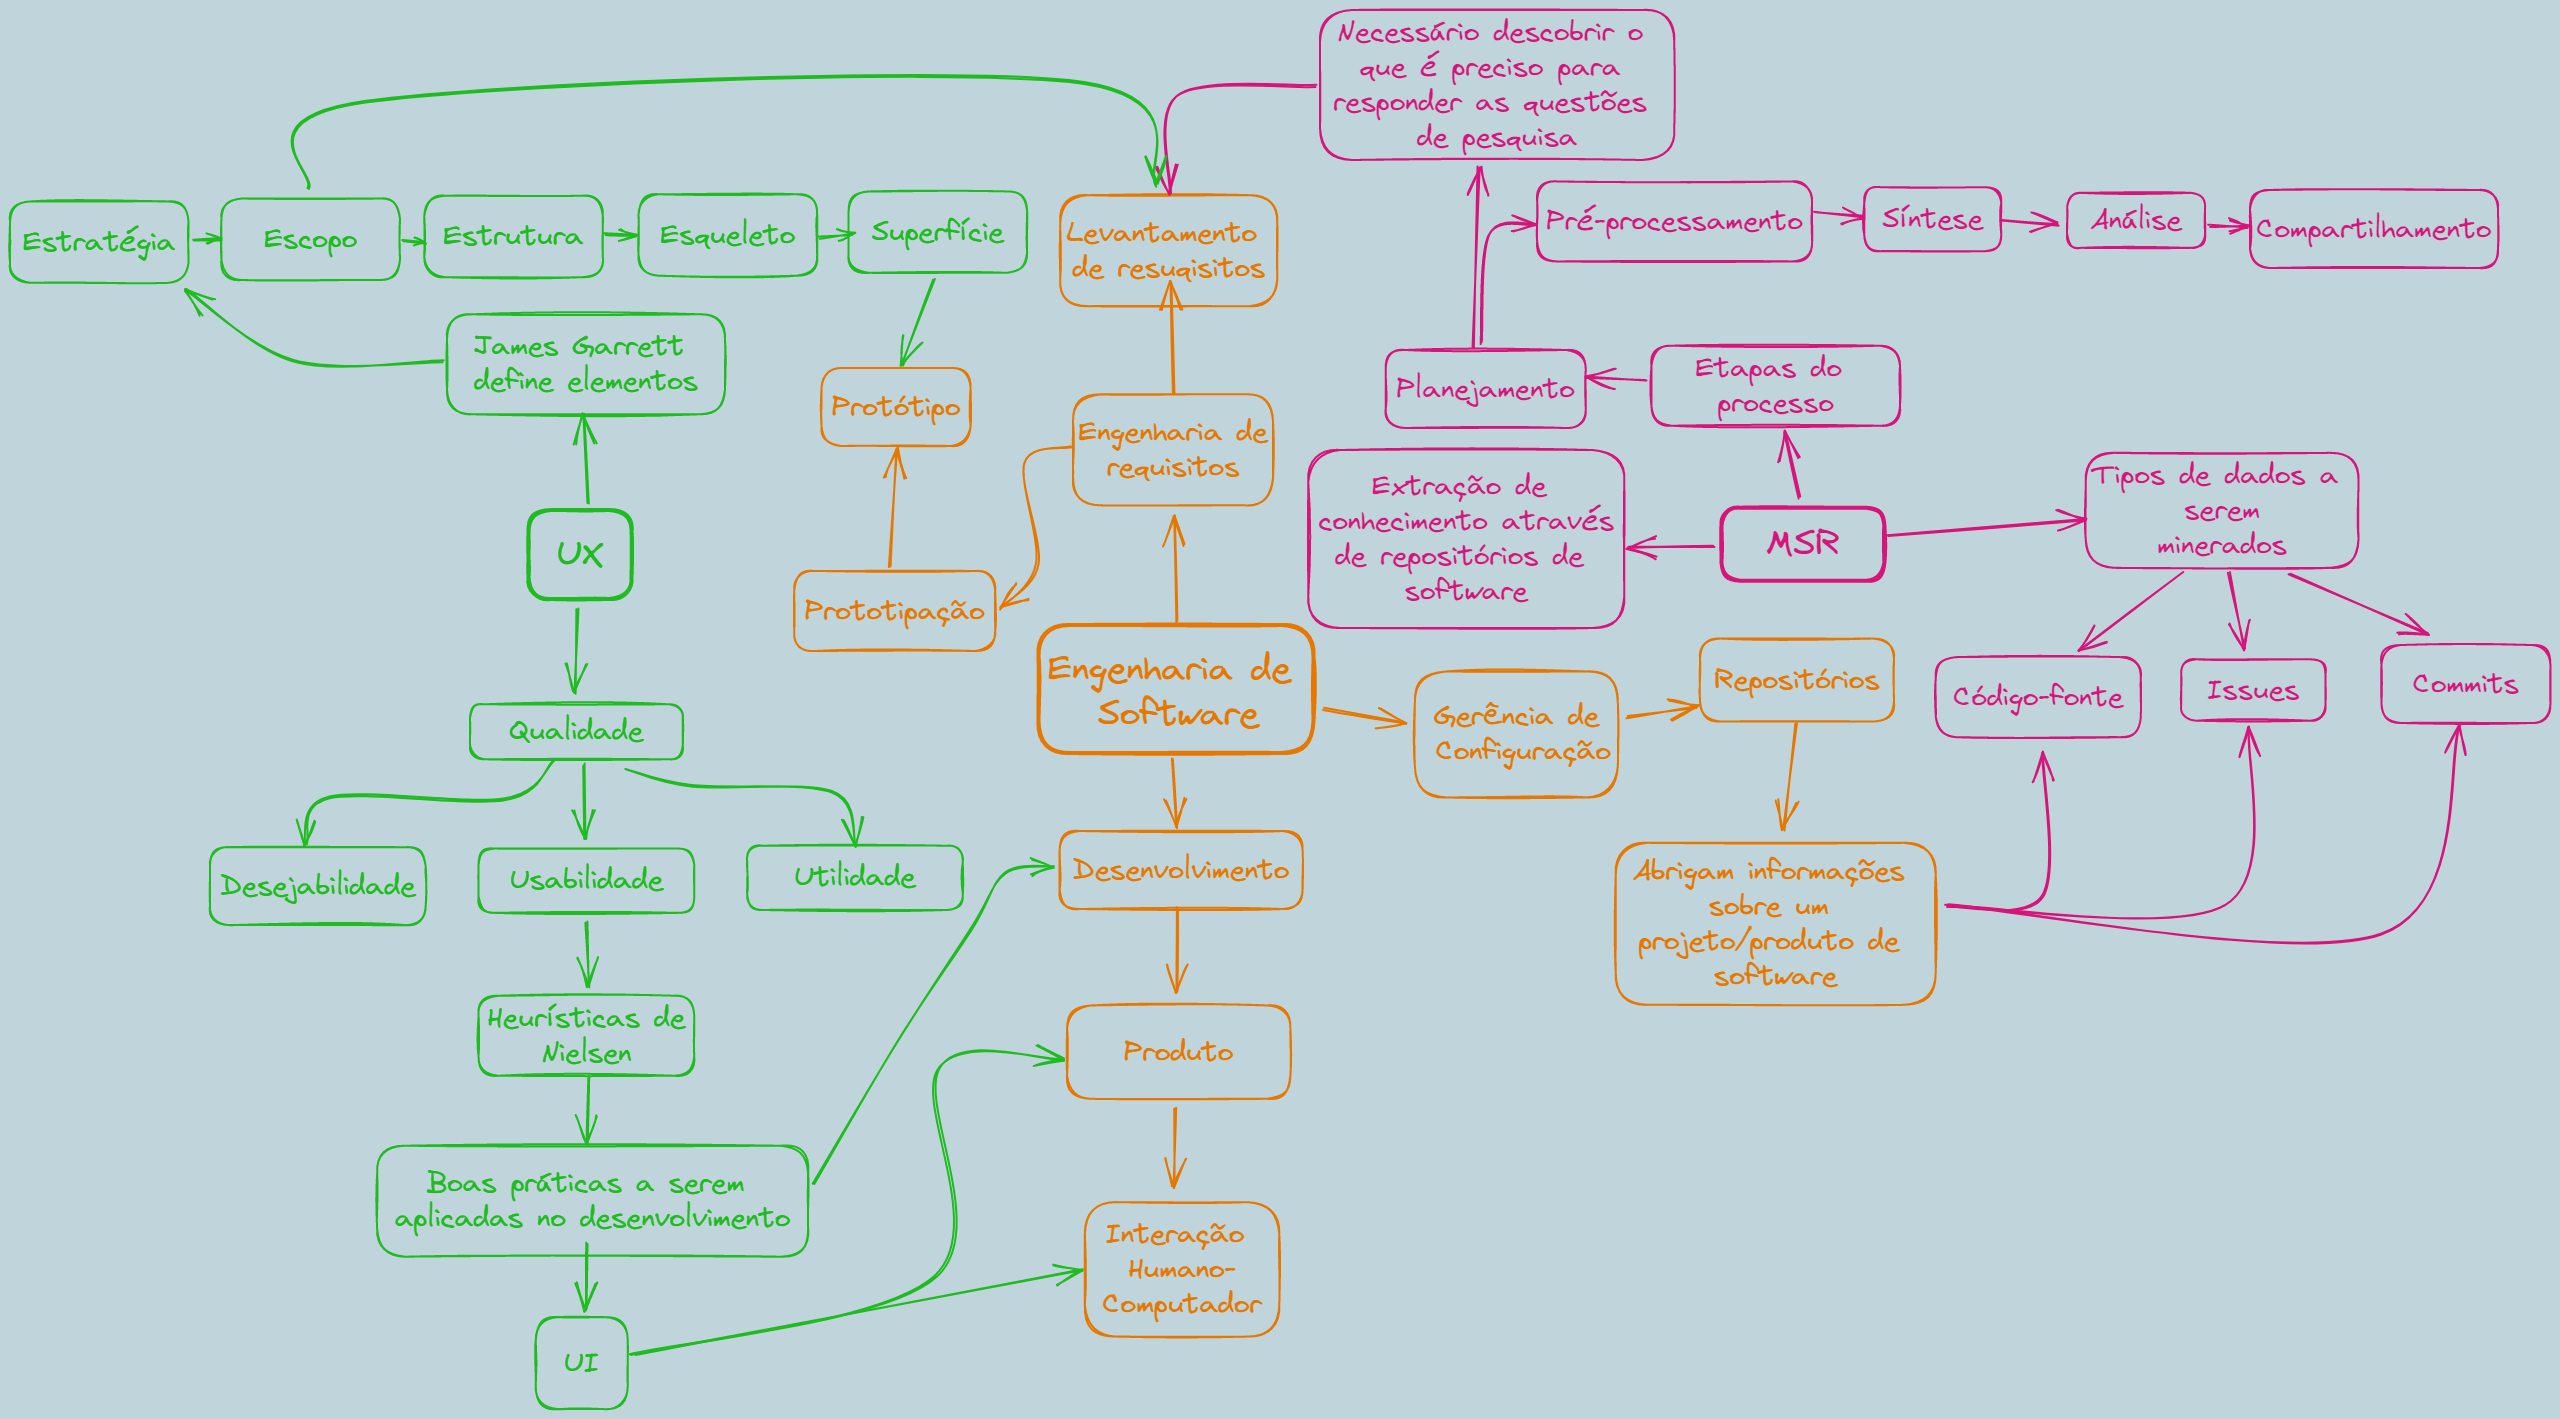
\includegraphics[width=1\textwidth]{img/mapa_mental.png}
    \caption{Mapa mental entre os conceitos de Engenharia de Software, MSR e UX}
    \label{fig:mapa_mental}
\end{figure}

\section{Questão 2}
% 2. Discussão. Por que precisamos de Engenharia de Software para (Inteligência Artificial, Aplicações Móveis, Web ou IoT) ? Discuta, em no mínimo três parágrafos e no máximo em cinco. Sua discussão deve ser baseada em, pelo menos, três artigos relacionados.
Sistemas de aprendizado de máquina (AM) são sistema de software que possuem componentes de Inteligência Artifical (IA) \cite{khomh2018software}. Dado o crescimento do AM no domínio de software, o simpósio SEMLA (do inglês, \textit{Software Engineering for Machine Learning Applications}) foi criado com a finalidade de discutir soluções de Engenharia de Software (ES) para sistemas de AM. Na edição de 2018 do SEMLA, Khomh et al. identificou duas atividades de ES que precisam ser aplicadas no contexto de aprendizado de máquina, estas são: testes e verificação de acurácia dos sistemas.

O levantamento de requisitos em sistemas de aprendizado máquina possuem suas próprias particularidades e desafios, como por exemplo, os requisitos são vistos como hipóteses que devem ser testadas via experimentos \cite{wan2019does}. Requisitos de sistemas AM geralmente são especificados por métricas quantitativas que por vezes são desconhecidas pelas partes interessadas, caso a métrica não esteja clara para os objetivos de negócio, isso pode influenciar o cliente a acreditar que o sistema não entrega o que foi pedido  \cite{giray2021software}. Essas particularidades demonstram a necessidade de que as técnicas de levantamento de requisitos (processo indispensável na ES) sejam adaptadas aos contextos de sistemas de AM.

Em um estudo de caso dentro da Microsoft, Amershi et al. descreveu as boas práticas da organização para o desenvolvimento de aplicações de aprendizado de máquina. Como resultado, os autores apontam a existência e necessidade de processos de ES presentes no \textit{workflow} de desenvolvimento de AM, entretanto foram necessárias adaptações desses processos para esse contexto. As três principais observações quanto a essas adaptações são: gerenciamento e descoberta de dados, customização e reuso, e modularidade \cite{amershi2019software}.


\section{Questão 3}
% 3. Proposta. Proponha uma abordagem que combine o Scrum mais o Shape UP considerando squads de produto e de apoio a produtos.
Scrum é uma metodologia ágil amplamente usada no desenvolvimento de software. Entretanto, podemos combinar técnicas ao Scrum de forma a extrair o máximo proveito da estratégia. A seguir será definida uma abordagem da combinação de conceitos do Shape Up (processo de desenvolvimento da Basecamp) ao Scrum, considerando \textit{squads} de produto e de apoio a produtos.

O processo do Scrum tradicionalmente (figura \ref{fig:scrum}) possui \textit{Sprints} iterativas que visam cumprir os objetivos levantados durante a \textit{Sprint Planning}. Uma adição proposta às \textit{squads} de produto, é a atividade de ``Cool Down'' definida no Shape Up, dessa forma a equipe tem previsto um tempo que será empregado para correção de bugs, refatoração e estudos (pagamento de dívida técnica), sem a necessidade de encaixar essas tarefas durante o ciclo de desenvolvimento de uma nova funcionalidade. Pode-se também variar a periodicidade de \textit{Sprints Cool Down} (SCD), ou seja, dependendo da necessidade da equipe, as SCDs podem ocorrer em alternância com a \textit{Sprint} comuns, ou a cada duas \textit{Sprints} comuns, por exemplo. Para impedir que apenas SCDs sejam realizadas, para esta proposta fica como regra o impedimento da realização SCDs consecutivas, ou seja, qualquer planejamento em que uma SCD preceda outra deve ser vetado. Importante pontuar que as \textit{Sprints Cool Down} possuem o mesmo \textit{timebox} que uma \textit{Sprint} comum, respeitando então a definição tradicional do Scrum. 

\begin{figure}[ht]
    \centering
    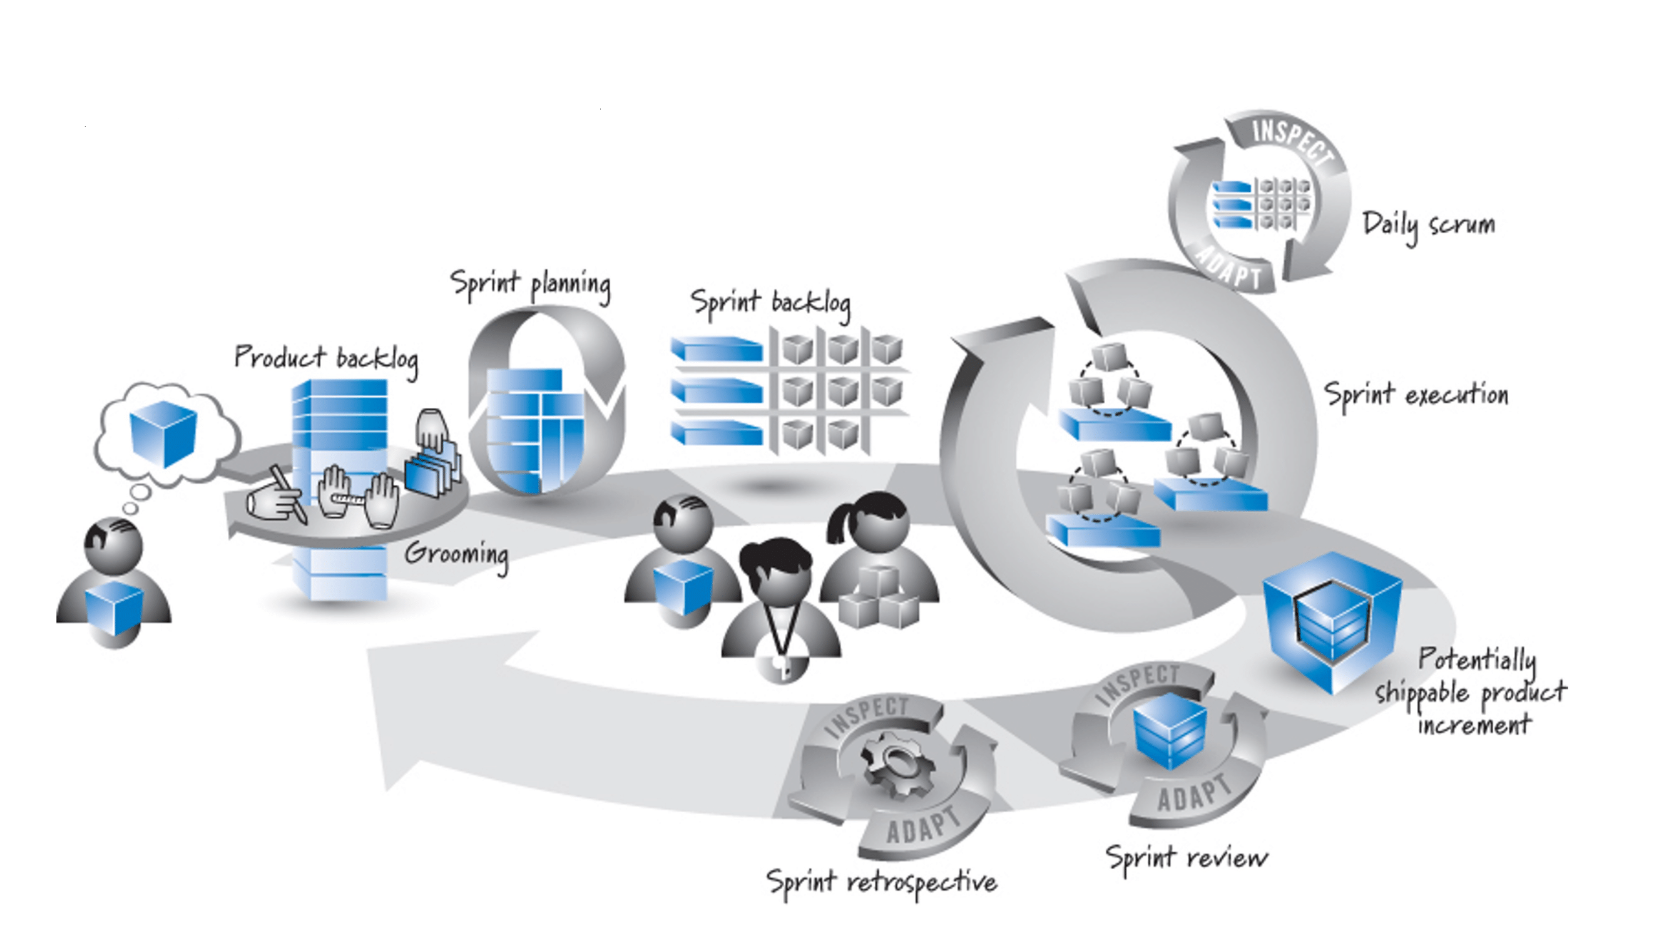
\includegraphics[width=0.8\textwidth]{img/scrum.png}
    \caption{Ilustração do processo tradicional do Scrum.}
    \label{fig:scrum}
\end{figure}

Outro conceito do Shape Up que pode beneficiar o Scrum (tanto \textit{squads} de produto como as de apoio ao produto) é o tamanho dos times. A opção por times menores facilita a sua autonomia. Como regra do Scrum, um profissional de cada área necessário para implementação deve compor a equipe. Portanto, por muitas vezes o número do Shape Up (dois desenvolvedores e um designer) pode não ser satisfatório as regras do Scrum, porém reduzir ao máximo a quantidade de pessoas dentro do time e criar times focados em objetivos (diferentes \textit{squads}) pode ser uma vantagem no desenvolvimento do produto.

Para o \textit{Product Backlog}, o Scrum define o processo de \textit{Grooming} responsável pela criação, refinamento, estimativas e priorização de estórias. Um conceito do Shape Up que pode ser adicionado a essa etapa do Scrum é a atividade de \textit{Pitch}. Além das tradicionais tarefas relacionadas as estórias, a estratégia do \textit{Pitch} pode ser adicionada a fim de enriquecer os requisitos. Ao contrário do Shape Up, todo o time seria encarregado dessa atividade. O \textit{Pitch} pode ser visto nesse caso como um acréscimo ao Scrum no sentido de auxiliar o entendimento do produto, no qual os integrantes da equipe, podem já em um primeiro momento, adicionar, por exemplo, esboços da solução. Ao chegar o momento de desenvolver dada funcionalidade, que foi contemplada pelo \textit{Pitch}, os desenvolvedores já teria uma melhor noção de como iniciar o desenvolvimento, possivelmente aumentando a produtividade do time.

Um esboço do processo proposto é mostrado na figura \ref{fig:scrum_shapeup}.
\begin{figure}[ht]
    \centering
    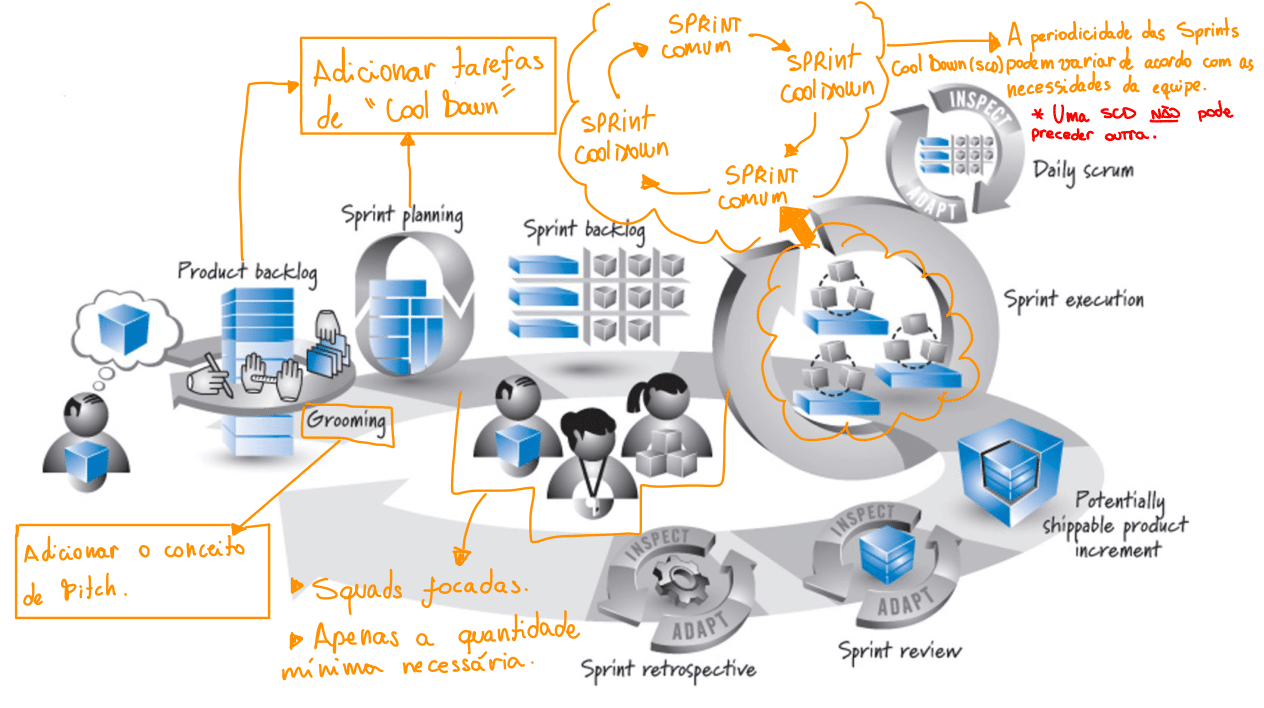
\includegraphics[width=0.8\textwidth]{img/scrum_shapeup.pdf}
    \caption{Processo proposto da combinação Scrum e Shape Up}
    \label{fig:scrum_shapeup}
\end{figure}

\section{Questão 4}
% 4. Defender or Detractor. Considerando o artigo "Benefitting from the Grey Literature in Software Engineering " disponível no AVA: argumente, em no mínimo três parágrafos e no máximo em cinco, as vantagens ou desvantagens do método e de seu uso. Você pode escolher uma posição de defender ou detractor. Deixe claro no início da resposta que posição escolheu adotar. Lembrando que seus argumentos devem ser referenciados.
A literatura cinza (da sigla em inglês, GL) é de grande utilidade como fonte de conhecimento, nesta seção serão apresentados argumentos a fim de apresentar os benefícios da GL com base no estudo ``Benefitting from the Grey Literature in Software Engineering'' \cite{garousi2020benefitting}. No dia-a-dia do desenvolvimento de software é comum, enquanto profissionais da área, depararmos com conceitos desconhecidos. Para isso, o mais comum é buscar conhecimento em fontes que entregam a informação de maneira pragmática e que seja de simples acesso, normalmente fontes de literatura cinza. A GL é um formato de literatura que não passou pelo processe formal de revisão por pares, e essa característica que faz com que esse tipo de literatura seja tão acessível.

Publicar em grandes revistas, conferências e outros canais da literatura branca é uma tarefa que demanda tempo e esforço, uma vez que esses canais precisam manter a qualidade dos textos publicados. Isso impede que pessoas, que não fazem parte e não estão habituadas com a escrita científica, possam publicar suas experiências. Muitas vezes, essas mesmas pessoas estão diretamente conectadas com o estado da prática de determinados assuntos, isso significa que a barreira da publicação (da literatura branca) pode impedir a disseminação de conteúdos valiosos sobre a realidade da indústria. Sendo assim, a literatura cinza combate essa barreira democratizando o acesso e publicação de conhecimento para qualquer pessoa que desejar compartilha-lo. 

Uma das desvantagens e preocupações intrínsecas a GL é qualidade e veracidade do que se é publicado. Garousi et al. inclusive cita Williams and Rainerqunato que afirmam que os materiais oriundo da GL precisam ser rigorosos, relevantes, bem escritos e baseados em experiência para serem considerados confiáveis para pesquisadores de Engenharia de Software \cite{williams2017toward}. Portanto, a qualidade acessível da GL não impede a descoberta de literatura válida. 

No âmbito científico ao realizar tarefas de sistematização de determinado assunto por meio da literatura cinza, se faz necessário o alto rigor quanto a qualidade do estudo, a fim de apresentar resultados verídicos. Entretanto, quanto a busca despretensiosa e cotidiana, que também necessita de dados confiáveis, possuem um rigor menor. Mesmo assim é possível verificar a fonte. Existem grandes canais de literatura cinza que são de vasta utilidade para o profissionais e pesquisadores da Engenharia de Software, como por exemplo a plataforma Medium que possui perfis oficiais de grandes organizações como a Netflix.

Comumente, a literatura branca costuma trazer estudos primários contendo o estado da arte de determinado assunto. Isso é de extrema importância para a evolução da Engenharia de Software (ES). Contudo, conhecer o estado da prática é indispensável dentro da ES. A natureza da literatura cinza é que seus autores são praticantes da indústria de ES, isso significa que a GL é uma fonte valiosa para conhecer o que a indústria está aplicando. Dito isso, a GL precisa fazer parte do meio científico da Engenharia de Software, assim como faz parte do cotidiano de vários profissionais da área.









\bibliographystyle{sbc}
\bibliography{refs}
\end{document}
